\documentclass[a4paper,UKenglish,cleveref,thm-restate]{lipics-v2021}
\usepackage{booktabs}
\nolinenumbers


\title{Range Minimum Queries: Analysis of Space-Time Trade-offs}
\author{Tamer Emad}{Karlsruhe Institute of Technology, Germany}{}{}{}
\authorrunning{Tamer Emad}
\hideLIPIcs

\begin{document}
\maketitle

\section{Introduction}
This report presents an empirical evaluation of several Range Minimum Query (RMQ) implementations. The objective is to analyze the trade-off between the auxiliary space required for preprocessing and the time complexity of subsequent queries. The submitted work consists of a C++ benchmarking suite (\texttt{main.cpp}) with the different implementations, the generator (\texttt{input-generator}) used to create the input data for the benchmarking, this report, along with the plots, visualizing the relationship between input size $n$, memory consumption, and query latency.

\section{Methods}
The RMQ problem is defined as: For a given array $a[N]$ of size N, and a query $q: [l, r]$ (or rather a large number of them), the RMQ is finding the minimum value within range $[l, r]$, for each query $q$. There is a wide spectrum of approaches to this problem, from naive linear scans to advanced data structures. This report implements and compares a sample of them.

\subsection{Implemented Algorithms}

\begin{itemize}
    \item \textbf{Naive Approach}: No preprocessing; computes the minimum via a linear scan for every query. Only a pointer to the array is stored.
    \item \textbf{Pointer-Based Segment Tree}: Is a variant of segtrees where each Node is constructed as a struct with pointers to the left and right child, and ints containing the min value and the range cover. The tree is built recursively on initiate. This implementation is easily extensible for more complex problems than RMQ. 
    \item \textbf{Optimized Segment Tree}: Is the more optimized implementation, getting rid of pointers and other variables and only storing a single, $2N$ sized array. where each node $i$ is a parent of $2i$, $2i+1$. This brings much better cache utilization.
    \item \textbf{Sqrt Decomposition}: Stores the answers (RMQ) for $\sqrt{N}$ blocks, each of size $\sqrt{N}$. Where every query needs to sweep a maximum of $2\sqrt{N}$ plain elements, and $\sqrt{N}$ blocks.
    \item \textbf{Prefixed Sqrt Decomposition}: Is a Prefix-optimized variant, where additionally the prefix and \textbf{suffix} minima of each block are also stored in two arrays of size $N$. Which eliminates the need for plain element sweeping.
    \item \textbf{Multilevel Sqrt Decomposition}: Furthermore, this is an optimization where a second Sqrt Decomposition is implemented on the blocks array of the first. While also making the first array's block size smaller $\sqrt{\sqrt{N}}$. This implementation offers more speedup in query time as the maximum number of blocks sweeped per query is $\sqrt{|blocks_1|} = N^{3/8}$.
    \item \textbf{Sparse Table}: Which is (using power-of-two intervals) to store the minimum. Where any query range $[l, r]$ is solved as the min between exactly two cells in the sparse table. 
    \item \textbf{Cartesian Trees}: Constructs a binary tree where the root is the minimum element of the array and its children are the Cartesian trees of the left and right subarrays. This transforms the RMQ problem into a Lowest Common Ancestor (LCA) problem, where the minimum of range $[l, r]$ is the LCA of the nodes corresponding to indices $l$ and $r$.
    \item \textbf{Brute-Force Precomputation}: Pre-calculates every possible answer in an $n \times n$ matrix.
\end{itemize}

The theoretical complexities of these methods are summarized in Table 1. And the application of the complexities to this particular problem task instance.

\begin{table}[h]
\centering
\caption{Theoretical Complexities and Total Execution Time ($n=10^7, Q=2 \cdot 10^6$)}
\label{tab:theoretical_complexities}
\begin{tabular}{lllll}
\toprule
\textbf{Algorithm} & \textbf{Space} & \textbf{Build Time} & \textbf{Query Time} & \textbf{Total Expected Time} \\ \midrule
Naive & $O(1)$ & $O(1)$ & $O(n)$ & $\approx 8000.0\text{ s}$ \\
Segment Tree (opt.) & $O(n)$ & $O(n)$ & $O(\log n)$ & $\approx 22.4\text{ ms}$ \\
Segment Tree (Pointers) & $O(n)$ & $O(n \log n)$ & $O(\log n)$ & $\approx 110.4\text{ ms}$ \\
PreCompute Answers & $O(n^2)$ & $O(n^2)$ & $O(1)$ & $\approx 40000.0\text{ s}$ \\
Sparse Table & $O(n \log n)$ & $O(n \log n)$ & $O(1)$ & $\approx 92.8 \text{ ms}$ \\
Sqrt Blocks & $O(\sqrt{n})$ & $O(n)$ & $O(\sqrt{n})$ & $\approx 2644.0\text{ ms}$ \\
Sqrt Blocks (prefix)  & $O(n)$ & $O(n)$ & $O(\sqrt{n})$ & $< 2644.0\text{ ms}$ \\
Multilevel Sqrt Blocks  & $O(n)$ & $O(n)$ & $O(n^{3/8})$ & $\approx 337.3\text{ ms}$ \\
Cartesian Tree (LCA) & $O(n \log n)$ & $O(n \log n)$ & $O(1)$ & $\approx 92.8\text{ ms}$ \\ \bottomrule
\end{tabular}
\begin{flushleft}
\small \textit{Assumption: Calculations assume 2500 operations take $\approx 1\text{ ns}$ (2.5 GHz). Total Time = Build Time + (Query Time $\times Q$).}
\end{flushleft}
\end{table}

According to the theory, the fastest methods are those achieving $O(1)$ query time, while the smallest is the Naive method. However, when also accounting for the build up / precompute time, the optimized segment tree is the smallest theoretically (for this exact problem constraints), as it takes $O(n)$ to build and only $Q \times \log n$ total query time.

\section{Results}
\begin{figure}[h]
    \centering
    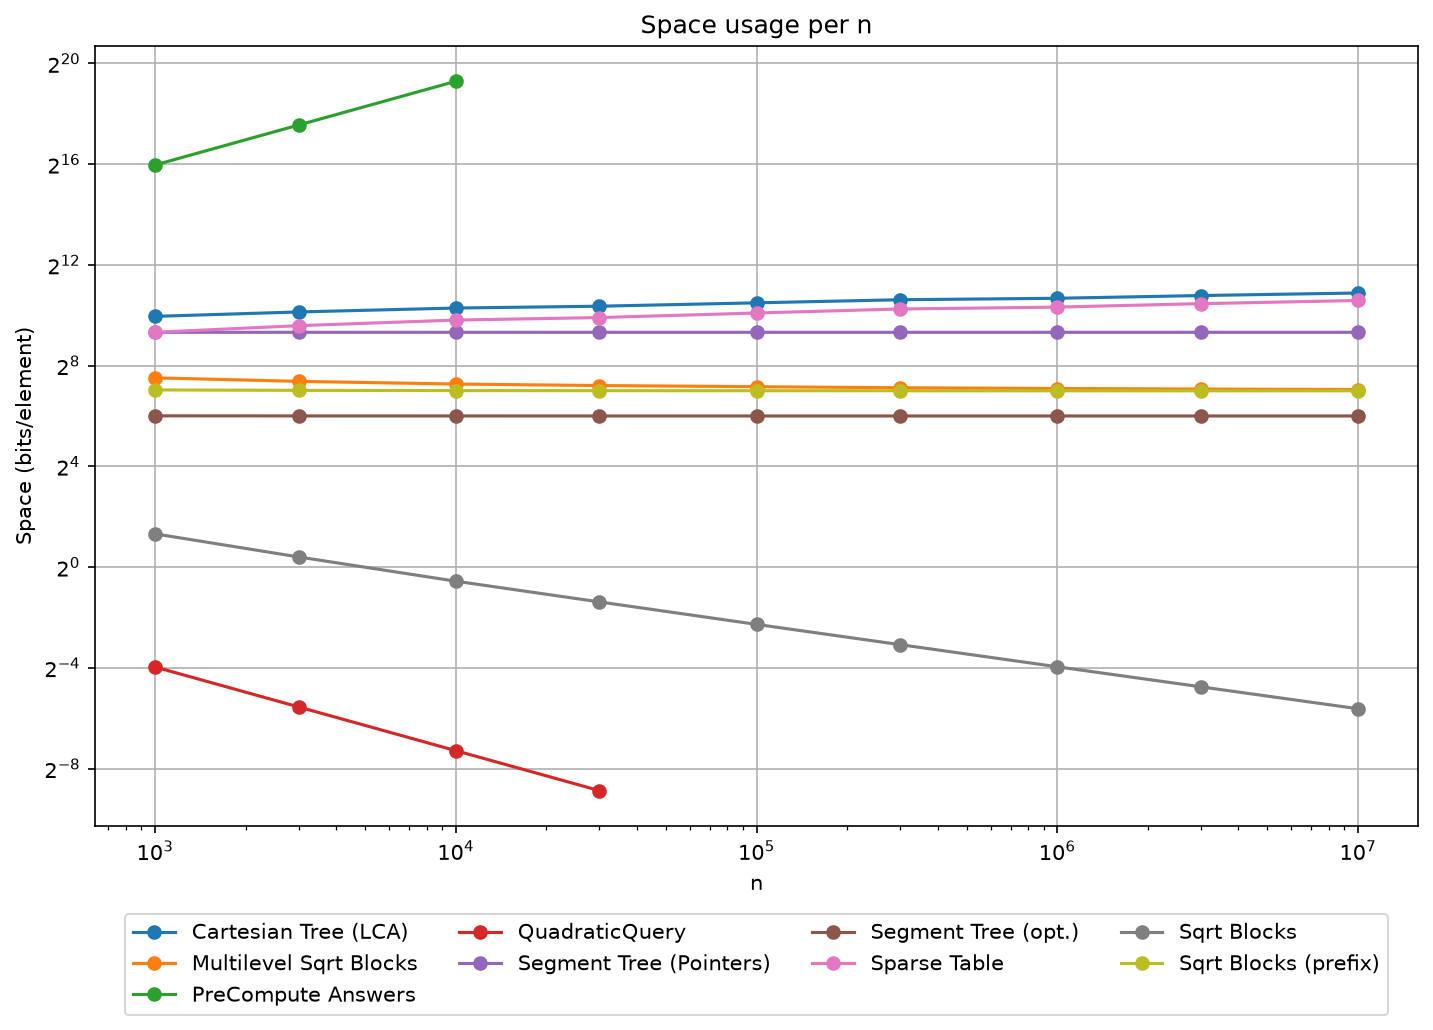
\includegraphics[width=.8\linewidth]{../plots/space.png}
    \caption{Space usage per element relative to input size $n$.}
    \label{fig:space}
\end{figure}
\begin{figure}[h]
    \centering
    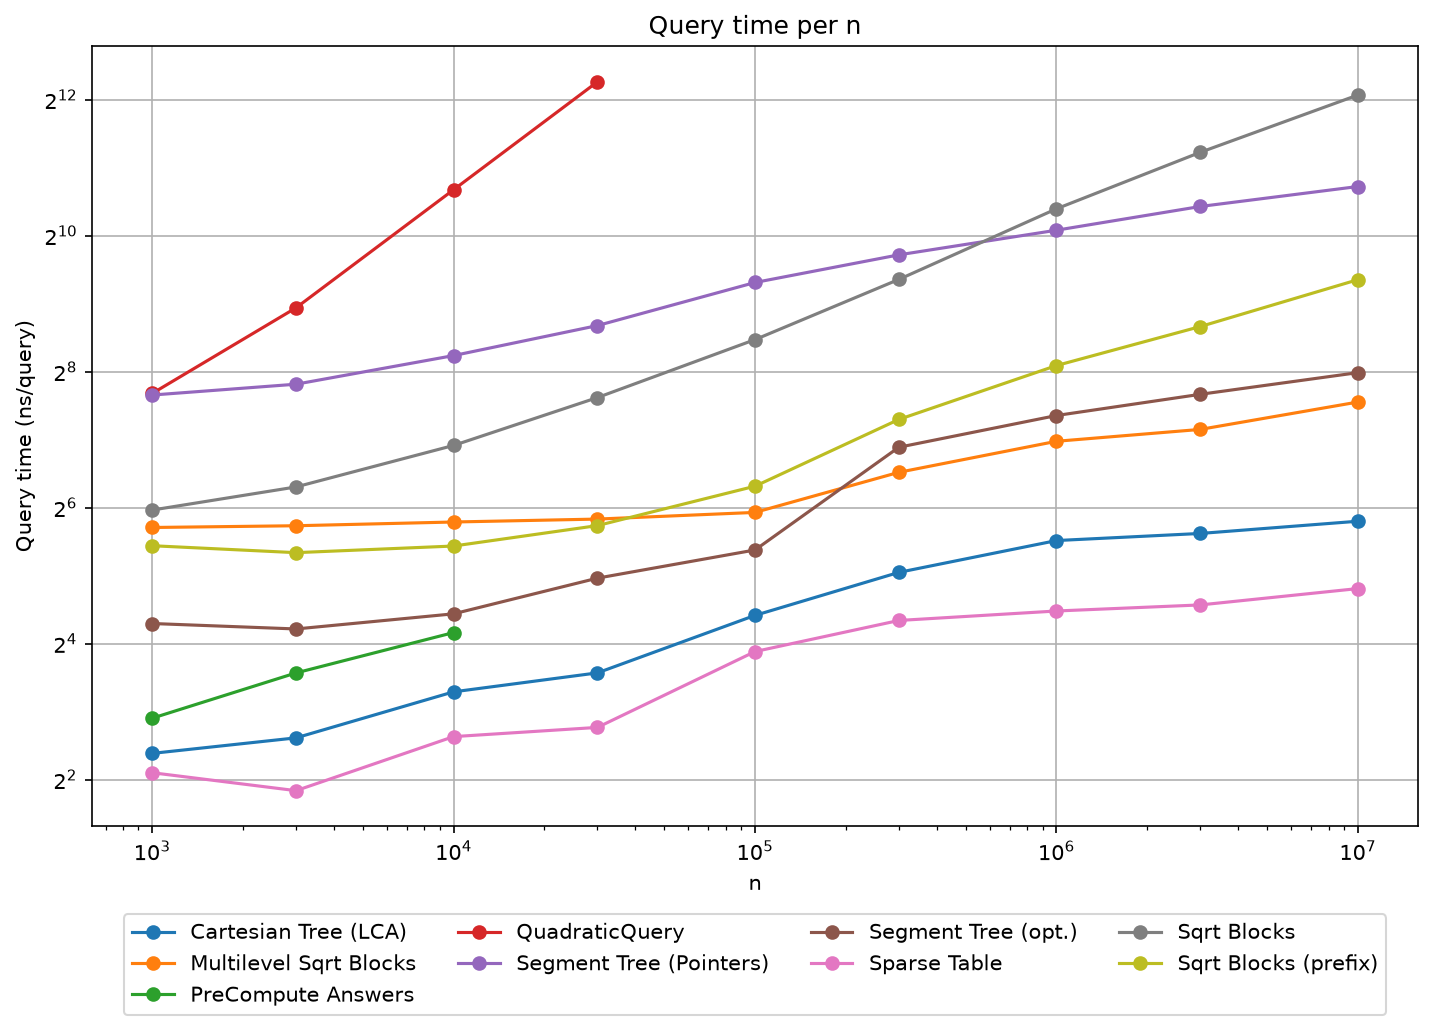
\includegraphics[width=.8\linewidth]{../plots/query_time.png}
    \caption{Query time (ns/query) as a function of input size $n$.}
    \label{fig:time}
\end{figure}
\begin{figure}[h]
    \centering
    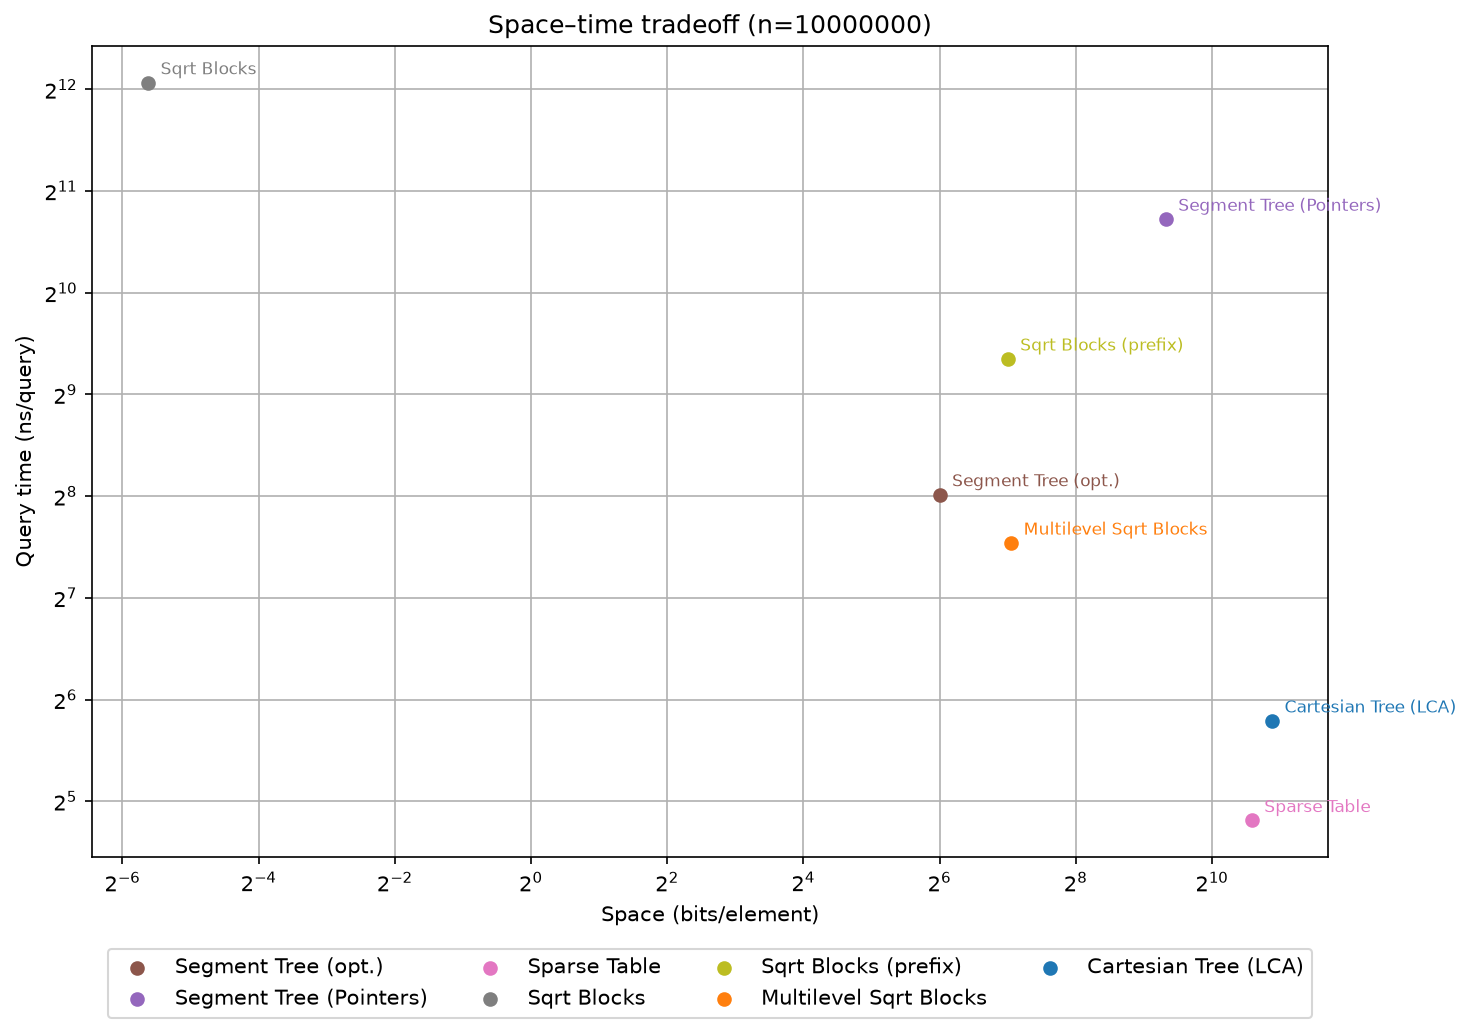
\includegraphics[width=.8\linewidth]{../plots/space_time_tradeoff.png}
    \caption{The space-time trade-off for $n=10^7$ elements.}
    \label{fig:tradeoff}
\end{figure}

\subsection{Analysis of Results}
The empirical results generally align with theoretical expectations. However, there is a constant factor of $0.5$ less than expected in theory and this is probably due to randomization of the input instead of worst case. as well as a combination of factors from compiler optimization and caching. In \cref{fig:time}, the Naive approach (QuadraticQuery) shows the steepest growth, while Sparse Tables and Cartesian Trees maintain a nearly flat line, confirming $O(1)$ query time. Similarly, \cref{fig:space} confirms that the PreCompute method grows quadratically, while the Naive approach uses negligible space. Interestingly, the Multilevel Sqrt is the lowest sloped line in \cref{fig:time} where it even crosses the optimized segment tree to perform better at $N > 10^5$ this shows that it is optimized more for this range of inputs. whereas, in the lower $N<10^4$ it performs even worse than the prefixed Sqrt Blocks. The segment tree is expected to overtake any Sqrt Decomposition algorithm with large enough $N$. Unless maybe it is a fractal Sqrt Decomposition?

\paragraph{Space and Time Fidelity}
Numerically, the space usage matches the theory closely. The Sparse Table's usage grows linearly with $n$ (with a $\log n$ slope), while the Sqrt-based methods stay strictly within $O(n)$ limits. But there is still more variations in the constant factors which corrispond directly to how the algorithm is implemented (i.e. two pre and suf arrays for Sqrt Blocks). The query times are asymptotically correct, although constants differ; for instance, the pointer-based Segment Tree is noticeably slower than the array-based one due to pointer indirection and cache misses.

\paragraph{Pareto Optimality}
Referring to \cref{fig:tradeoff}, the Pareto-optimal algorithms, providing the best speed for a certain space budget, are the \textbf{Sparse Table} and, only a factor of 2 slower, the \textbf{Cartesian Tree} for time efficient requirements, Whereas \textbf{Sqrt Blocks} is best viable for low-memory environments. Meeting in the middle, with a more balanced trade-off at $O(N)$ memory and $O(\log N)$ time per query, is the \textbf{Segment Tree (opt.)} alongside the \textbf{Multilevel Sqrt Blocks}. At the end, \textbf{Sparse Table} is the practically optimal choice as $O(n \log n)$ space is usually acceptable for modern memory capacities in exchange for constant-time queries.
It is also worthy to note that the Multilevel Sqrt drops query time by x4 while keeping the efficient space usage that is due to low space usage from the 2nd level Sqrt decomposition where the time gain is much higher. Also notable, is how the pointers Segment tree takes up ~ 8x more space than the optimized one, as every Node stores the values, the range left and right as well as the pointers to the children. This can be further optimized but it was not pursued further in this report. Also it might be interesting to test how a trinary (or d-nary) tree might work by doing a threeway (d-way) split in each Node.

\paragraph{Absolute Performance and Bottlenecks}
The fastest methods operate in the range of a few dozen nanoseconds per query (exactly 28.0ns). At this scale, the bottleneck is no longer the algorithmic complexity, but rather the hardware architecture. Specifically, \textbf{L1/L2 cache misses} become the primary limit.

\end{document}
